\documentclass[12pt]{article} % \documentclass{} is the first command in any LaTeX code.  It is used to define what kind of document you are creating such as an article or a book, and begins the document preamble

\usepackage{amsmath} % \usepackage is a command that allows you to add functionality to your LaTeX code

\usepackage[papersize={216mm,330mm},tmargin=20mm,bmargin=20mm,lmargin=20mm,rmargin=20mm]{geometry}
\usepackage[english]{babel}
\usepackage[utf8]{inputenc}
\usepackage{amsmath,amssymb,mathabx,amsthm}%\for eqref
\usepackage{lscape}
\usepackage{graphicx}
\usepackage{tikz}
\usepackage[colorinlistoftodos]{todonotes}
\usepackage{fancyhdr}
\usepackage{hyperref} %creat hyperlink
\hypersetup{
    colorlinks=true,
    linkcolor=blue,
    filecolor=magenta,      
    urlcolor=cyan,
    pdftitle={Overleaf Example},
    pdfpagemode=FullScreen,
    } %set up a hyperlink to be in blue 
\newtheorem{theorem}{Theorem}
\newtheorem{definition}{Definition}[section]
\newtheorem{prop}{Proposition}[section]
\newtheorem{lemma}{Lemma}[section]

\pagestyle{fancy}
\fancyhf{}
\setlength\parindent{0pt} % noindent for the whole document.
\renewcommand{\baselinestretch}{1.2} % increase the distance between line.

\DeclareMathOperator{\SL2}{\text{SL}_2(\mathbb{R})}
\DeclareMathOperator{\sl2z}{SL_2(\mathbb{Z})}

\DeclareMathOperator{\SO}{SO_2(\mathbb{R})}
\DeclareMathOperator{\uH}{\mathfrak{H}}



\title{CHAPTER I : $\SL2$} % Sets article title
\date{\today} % Sets date for date compiled

% The preamble ends with the command \begin{document}
\begin{document} % All begin commands must be paired with an end command somewhere
\maketitle % creates a title using the information in the preamble (title, author, date)
In this chapter, I will give an exposition on the structure of $\SL2$ as the spaces of lattice, this space
plays the role of a toy model before exploring the space of lattice in the higher rank. The exposition follows
the paper \cite{} and  \cite{} closely.
\section{$\SL2$ and its action on the upper half plane $\uH$}
A priori, the upper half plane
\[\uH = \left\lbrace z: \Im z >0 \right\rbrace \subset \mathbb{C}\]
has no group structure on its. However, we will show below that it can identify topologically with the space
with the space of cosets $\SO\backslash\SL2$, and thus we can study the spaces $\uH$ via the spac of lattices $\SO\backslash\SL2$.
We define the action of $G= \SL2$ on $\uH$ as follows
\[
  \begin{bmatrix}a & b \\ c & d\end{bmatrix} \circ (z) = \frac{az + b}{cz + d}
\]
\begin{prop}
  The group \(SL_{2}(\mathbb{R})\) stabilizes \(\mathfrak{H}\) and acts transitively on it. In particular,
  \[
    \begin{bmatrix}1 & x \\ 0 & 1\end{bmatrix}\begin{bmatrix}\sqrt{y} & 0 \\ 0 & \frac{1}{\sqrt{y}}\end{bmatrix}(i) = x + iy \quad (\text{for } x \in \mathbb{R}, \, y > 0)
  \]
  Further, for \(g = \begin{bmatrix}a & b \\ c & d\end{bmatrix} \in SL_{2}(\mathbb{R})\) and \(z \in \mathfrak{H}\),
  \[
    \text{$\Im$}\,g(z) = \frac{\text{$\Im$}\,z}{|cz + d|^2}.
  \]
\end{prop}
\begin{proof}
  The first formula is clear. The second formula would imply that the upper half-plane is stabilized. Compute directly:
  \[
    2i \cdot \text{$\Im$} \left( \begin{pmatrix} a & b \\ c & d \end{pmatrix} (z) \right) = \frac{az + b}{cz + d} - \frac{d\overline{z} + b}{c\overline{z} + d} = \frac{(az + b)(c\overline{z} + d) - (a\overline{z} + b)(cz + d)}{|cz + d|^2}
  \]
  \[
    = \frac{adz - bc\overline{z} - bcz + ad\overline{z}}{|cz + d|^2} = \frac{z - \overline{z}}{|cz + d|^2}
  \]
  since \( ad - bc = 1 \).
\end{proof}
The point $z = i$ is special, in the sense that its stability group is the orthogonal group $K =\SO$. Indeed, for any \(g = \begin{bmatrix}a & b \\ c & d\end{bmatrix} \in SL_{2}(\mathbb{R})\)  we have
that
\[g \circ i = i \Leftrightarrow \dfrac{ai+b}{ci+d }=i \Leftrightarrow a=d \text{ and } b = -c \]
Combinining with the fact that $ad-bc=1$, we must have $a^2 + b^2=1$. This implies that there is a $\theta$ such that $a = \cos\theta$ and $b = \sin \theta$.
Since $G$ acts on $\uH$ transitively, we know from group theory that there is a bijection between the collection of cosets of
$\text{Stab}(i)$ in $G$ and the orbits of $i$. In particular
\begin{prop}
  We have an isomorphism of \(SL_{2}(\mathbb{R})\)-spaces
  \[
    \SO\backslash\SL2 \approx \mathfrak{H} \quad \text{via} \quad  SO(2)g \to g^{-1}(i)
  \]
  That is, the map respects the action of \(SL_{2}(\mathbb{R})\), in the sense that
  \[
    (\SO g)\cdot h \;\longrightarrow\; h^{-1}(g^{-1}i)
  \]
\end{prop}
\begin{proof}
  This is because of \textit{associativity}:
  \[
    (\SO g)\cdot h  = (\SO)\cdot (gh)  \;\longrightarrow\; (gh)^{-1}(i) = h^{-1}(g^{-1}(i))
  \]
  giving the result.
\end{proof}
\section{Fundamental domain for $\Gamma = SL_2(\mathbb{Z})$ on $\mathfrak{H}$}
Here is a picture of the fundamental domain $\mathfrak{H}/\Gamma$.
\[
  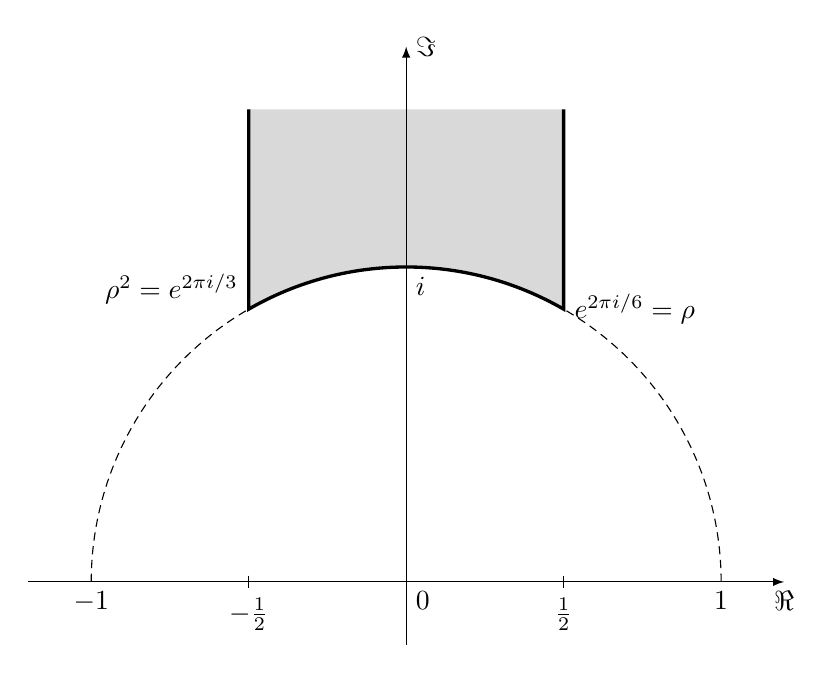
\begin{tikzpicture}[scale=4]
    \draw[densely dashed] (1,0) arc (0:60:1) (-1,0) arc (180:120:1);
    \draw[very thick, fill=gray!30] (.5,1.5) --node[right, pos=1]{$e^{2\pi i/6}=\rho$} (60:1) arc (60:120:1)
    --node[left, pos=.1]{$\rho^2=e^{2\pi i/3}$} (-.5,1.5);
    \draw[-latex] (-1.2,0) -- (1.2,0)node[below]{$\Re$};
    \draw[-latex] (0,-.2) -- (0,1.7)node[right]{$\Im$};
    \path(-1,0) --node[below, pos=0]{$-1$}node[below right, pos=.5]{0}node[below, pos=1]{1} (1,0)
    (0,1)node[below right]{$i$};
    \draw(-.5,.02)--(-.5,-.02)node[below]{$-\frac{1}{2}$}(.5,.02)--(.5,-.02)node[below]{$\frac{1}{2}$};
  \end{tikzpicture}\]
The goal of this section is to prove that under the action of the $\Gamma = \sl2z$, we can "move"
every points on the upper half plane to a domain, under an equivalence given by a specific action.
This is similar to the fundamental domain given by the translation action of $\mathbb{Z}$ to $\mathbb{R}$ is the half-open
unit interval $[0,1)$. In general, this give a simpler description to the homogenous space of lattice.

Not that when we try to compute the fundamental domain of $\mathbb{Z}\backslash \mathbb{R}$, we have $\mathbb{Z}$ plays a role of
"discrete" subset of $\mathbb{R}$. We give a precise definition of discreteness as follows
\begin{definition}
  Let a group $G$ act continuously on a topological space $X$. A subset $\Gamma \subset G$ is called \textbf{discrete} if for any two compact subse
  $A,B$ in $X$, there are only finitely many $g \in \Gamma$ such that $g \circ A \cap B \ne \emptyset$.
\end{definition}
We will prove that the set
\[\Gamma = \sl2z = \left\lbrace \begin{bmatrix}
    a & b \\
    c & d
  \end{bmatrix} \in \SL2: a, b, c, d \in \mathbb{Z}\right\rbrace\]
is a discrete subgroup of $G = \SL2$.
To prove this, we first need the following lemma
\begin{lemma}\label{lm2}
  Fix a real number $r>0$ and $0<\delta<1$. We denote $R_{r,\delta}$ the rectangle
  \[R_{r,\delta} = \left\lbrace z = x+iy: -r \le x \le r, 0 <\delta \le y \le \delta^{-1}\right\rbrace\]
  Then for any $\epsilon >0$ and any fixed set $\mathbb{S}$ of coset representatives for $\Gamma_\infty\backslash \Gamma$, there are finitely
  many $g \in \mathbb{S}$ such that $\Im(g\circ z)>\epsilon$ for some $z \in R_{r,\delta}$.
\end{lemma}
In the above lemma, the notation $\Gamma_\infty$ is defined to be the set
\[ \Gamma_\infty = \left\lbrace\begin{bmatrix}
    1 & n \\
    0 & 1
  \end{bmatrix}: n \in \mathbb{Z} \right\rbrace.\] It can be seen easily that this is the
stability group of $\infty$ in $\mathfrak{H}$.
\begin{proof}
  Let \( g = \begin{bmatrix} a & b \\ c & d \end{bmatrix} \). Then for \( z \in R_{r, \delta} \),
  \[
    \text{Im}(g \circ z) = \frac{y}{c^2 y^2 + (cx + d)^2} < \epsilon
  \]
  if \( |c| > (y \epsilon)^{-\frac{1}{2}} \). On the other hand, for \( |c| \leq (y \epsilon)^{-\frac{1}{2}} \leq (\delta \epsilon)^{-\frac{1}{2}} \), we have
  \[
    \frac{y}{(cx + d)^2} < \epsilon
  \]
  if the following inequalities hold:
  \[
    |d| > |c| r + (y \epsilon^{-1})^{\frac{1}{2}} \geq |c| r + (\epsilon \delta)^{-\frac{1}{2}}.
  \]
  Consequently, \(\Im(g \circ z) > \epsilon\) only if
  \[
    |c| \leq (\delta \epsilon)^{-\frac{1}{2}} \quad \text{and} \quad |d| \leq (\epsilon \delta)^{-\frac{1}{2}} (r + 1),
  \]
  and the total number of such pairs (not counting $(c, d) = (0, \pm 1), (\pm 1, 0)$) is at most $\frac{4(r+1)} {(\epsilon \delta)}$. This proves the lemma.
\end{proof}
It follows from Lemma 1.1.6 that $\Gamma = SL(2, \mathbb{Z})$ is a discrete subgroup of $SL(2, \mathbb{R})$. This is because:

\begin{enumerate}
  \item It is enough to show that for any compact subset $A \subset \mathfrak{h}$ there are only finitely many $g \in SL(2, \mathbb{Z})$ such that $(g \circ A) \cap A \neq \phi$;

  \item Every compact subset of $A \subset \mathfrak{h}$ is contained in a rectangle $R_{r,\delta}$ for some $r > 0$ and $0 < \delta < \delta^{-1}$;

  \item $((\alpha g) \circ R_{r,\delta}) \cap R_{r,\delta} = \phi$, except for finitely many $\alpha \in \Gamma_{\infty}$, $g \in \Gamma_{\infty}\backslash \Gamma$.
\end{enumerate}

To prove (3), note that Lemma \ref{lm2} implies that $(g \circ R_{r,\delta}) \cap R_{r,\delta} = \phi$ except for finitely many $g \in \Gamma_{\infty}\backslash \Gamma$. Let $S \subset \Gamma_{\infty}\backslash \Gamma$ denote this finite set of such elements $g$. If $g \not\in S$, then Lemma 1.1.6 tells us that it is because $\Im(g \circ z) < \delta$ for all $z \in R_{r,\delta}$. Since $\Im(\alpha g \circ z) = \Im(g \circ z)$ for $\alpha \in \Gamma_{\infty}$, it is enough to show that for each $g \in S$, there are only finitely many $\alpha \in \Gamma_{\infty}$ such that $((\alpha g) \circ R_{r,\delta}) \cap R_{r,\delta} \neq \phi$. This last statement follows from the fact that $g \circ R_{r,\delta}$ itself lies in some other rectangle $R_{r',\delta'}$, and every $\alpha \in \Gamma_{\infty}$ is of the form $\alpha =
  \begin{bmatrix}
    1 & m \\
    0 & 1
  \end{bmatrix}
  (m \in \mathbb{Z})$, so that
\[
  \alpha \circ R_{r',\delta'} = \{x + iy \mid -r' + m \leq x \leq r' + m, \, 0 < \delta' \leq \delta''^{-1}\},
\]

which implies $(\alpha \circ R_{r',\delta'}) \cap R_{r,\delta} = \phi$ for $|m|$ sufficiently large.

\end{document} % This is the end of the document